\documentclass[a4paper,zihao=5,UTF8,fontset=fandol]{../phyreport}
\usepackage{subcaption}
% \usetikzlibrary{decorations.pathmorphing}
\expName{用实验方法找出弹簧振子周期的表达式}
\expDate{2024}{4}{19}
\subDate{2024}{4}{26}
% \expAddr{致原楼207}

\begin{document}
\phyExpCover
\section{实验设计方案}
\subsection{实验目的}
\subsubsection{实验要求}
假设我们不知道弹簧振子的理论公式,用实验的方法(用实验数据)找出弹簧振子数学解析式。

\subsubsection{实验目的}
在实际工作中,我们会遇到一些新的物理现象,我们需要对物理现象进行研究,发掘它的规律,本实验的目的在于学习用实验方法找出物理规律的表达式,重点是学习研究问题的方法。
\subsection{研究思路}
本实验无原理,思考过程与一般不同,注重从现象、数据到规律的推导过程。采取以下步骤:
\begin{enumerate}
	\item 确定周期$T$与哪些因素有关
	\item 控制$k$不变,找出$T(m)$
	\item 控制$m$不变,找出$T(k)$
	\item 分析 $T(m)$ 和 $T(k)$,找出 $T(m,k)$ 解析式
	\item 确定系数
\end{enumerate}
关键点在于如何控制 $k$ 和 $m$,实验时不常如何选取,如何找出 $T(m)$ 和 $T(k)$,以及如何分析 $T(m)$ 和 $T(k)$。

\paragraph{确定周期$T$与哪些因素有关}

想要得到弹簧振子的周期公式,
首先观察实验中有哪些物理量,如 $T$、$m$、$k$,推断周期$T$与质量$m$和劲度系数$k$之间可能的关系。
实验中控制变量,分别改变质量$m$和劲度系数$k$,来观察它们对周期$T$的影响。

\subsection{实验原理}
\paragraph{量纲分析步骤}
\begin{enumerate}
\item 识别相关变量:首先,确定对研究问题具有影响的所有物理量。
\item 列出量纲方程:书写每个物理量的量纲表达式。例如,$T$的量纲是$T$,$m$的量纲是$M$,$k$的量纲可表示为$M/T^2$(因为$k= \text{力}/\text{位移}$,而力的量纲是质量乘以加速度)。
\item 建立量纲齐次方程:基于物理直觉或经验,假设一个可能的关系式,并确保方程两边的量纲相匹配。
\end{enumerate}
\paragraph{弹簧的有效质量}
一个均匀弹簧沿其长度振动时,有效质量是其实际质量的约三分之一。可以假设弹簧的每个部分都以不同的振幅振动。弹簧固定一端,另一端自由或连接质量。设\( \rho \) 是弹簧材料的密度,\( A \) 是横截面积,\( L \) 是弹簧长度,\( v(x) \) 是位置 \( x \) 处的速度。

弹簧的总动能可以表示为:
\begin{equation}
	K = \int_0^L \frac{1}{2} \rho A v(x)^2 \, dx
\end{equation}

由于速度沿弹簧长度非均匀分布,速度在弹簧自由端达到最大,我们可以进一步假设速度从固定端到自由端线性增加:
\begin{equation}
	v(x) = v_{\text{max}} \left(\frac{x}{L}\right)
\end{equation}

将代入速度到动能得:
\begin{equation}
		K = \int_0^L \frac{1}{2} \rho A \left(v_{\text{max}} \frac{x}{L}\right)^2 \, dx   = \frac{1}{2}\left( \frac{1}{3} \rho A L \right) v_{\text{max}}^2
\end{equation}

因此,总动能可以看作是由质量 \( \frac{1}{3} \rho A L \) 以速度 \( v_{\text{max}} \) 运动产生,即有效质量为 $m_{\text{eff}} = \frac{1}{3} m$

\subsection{实验仪器}
% \subsubsection{实验装置}
% \begin{figure}[H]
% 	%\tikzfig{coli.tikz}
% 	\centering
% 	\begin{tikzpicture}[font=\small]
% 		\draw[] (-3, 0) rectangle (3, -0.5);
% 		\draw[] (-2, 0) rectangle (-1.5, 6);
% 		\draw[] (2, 0) rectangle (1.5, 6);
% 		\draw[] (2,6) rectangle (-2, 6.5);
% 		\draw[] (0.5, 6) rectangle (-0.5, 5);
% 		\draw[decoration={coil,aspect=0.3,segment length=3mm,amplitude=3mm},decorate] (0,5) -- (0,3.5);
% 		\draw[] (0.3, 3.5) -- (-0.3, 3.5) -- (-0.5, 2.5) -- (0.5, 2.5) -- (0.3, 3.5);
% 		% 激光测距仪
% 		\draw[fill = white] (0.4, 1) rectangle (-0.4, -0.5);
% 		\draw[dashed] (0, 1) -- (0,3.5);
% 		\draw[fill=white] (0, 1) circle [radius=0.1];
% 		\draw[] (0.5, 0.9) -- (2.1, 0.9);
% 		\node[right] at (2.1, 0.9) {激光测距仪};
% 		\draw[] (2.1, 3) -- (0.6, 3);
% 		\draw[] (2.1,5.5) -- (0.6, 5.5);
% 		\node[right] at (2.1, 3) {砝码};
% 		\node[right] at (2.1, 5.5) {力传感器};
% 		\draw[] (2.1, 0.3) -- (2, 0.3);
% 		\node[right] at (2.1,0.3) {支架};
% 	\end{tikzpicture}
% 	\caption{实验装置示意图}
% \end{figure}
% \subsubsection{仪器列表}
本实验使用的仪器如下表所示:
\begin{table}[H]
	\centering
	\caption{选用仪器列表} \label{仪器列表}%
	\begin{tabular}{lll}
		\toprule
		仪器名称               & 型号      & 用途          \\
		\midrule
		850接口              & UI-5000 & 数据采集处理      \\
		计算机和PASCO Capstone & CI6874  & 数据采集平台、数据处理 \\
		力传感器               & -       & 测量力的大小      \\
		砝码(10-1000g)    & -       & 为弹簧提供拉力     \\
		激光测距仪              & -       & 测量弹簧伸长量     \\
		\bottomrule
	\end{tabular}
\end{table}
\longLine
\section{实验内容及具体步骤}
\subsection{控制 $k$ 确定$T(m)$}
\begin{enumerate}
	\item 在弹簧下方挂质量$m$砝码。
	\item 拉动弹簧,让其自由振动。
	\item 使用Capstone 软件$F-t$的图像,正弦曲线拟合,记录拟合的频率$\omega$。
	\item 改变$m$,重复上述操作。
	\item 确保在整个实验过程中使用相同的弹簧,以保证劲度系数 \(k\) 保持不变。
	\item 幂指数拟合,得 \(T\) 与 \(m\) 之间的关系。
\end{enumerate}

\subsection{控制$m$确定$T(k)$}
\begin{enumerate}
	\item 将激光测距仪固定在与弹簧伸长方向平行的位置上
	\item 挂上不同质量的砝码,使用激光测距仪测量弹簧伸长的距离
	\item 得到至少五组质量$M$与弹簧伸长量$\Delta x$的数据
	\item 选取同一质量$m$的砝码,对不同的弹簧使用Capstone 软件记录时间$t$对力$F$的图像,并使用正弦曲线拟合,记录拟合的频率$\omega$,计算周期 \(T\)
	\item 将收集到的数据(周期 \(T\) 和弹性系数 \(k\))绘制成图表。
	\item 幂指数拟合,得 \(T\) 与 \(k\) 之间的关系。
\end{enumerate}

\subsection{得到$T(m,k)$解析式}
通过综合 $T(m)$与$T(k)$,进一步量纲分析,找出$T(m,k)$解析表达式。

\longLine
\section{数据记录及数据处理}
\subsection{控制$k$确定$T(m)$}
选择一根弹簧,测量得到其质量 $m_0=21 \text{g}$,重力加速度取$g= 9.8 \text{m/s}^2$

\begin{table}[H]
	\centering
	\caption{控制 $k$ 记录 $F$ 与 $m$ 的关系}
	  \begin{tabular}{rrrrr}
		\toprule
		砝码质量$M$(g) & 有效质量$m$(g) & 所受力$F$(N) & 频率 $\omega $(rad/s)& 周期 $T$(s) \\
		\midrule
	  1000  & 21    & 1007  & 11.3  & 0.556  \\
	  1200  & 21    & 1207  & 10.3  & 0.610  \\
	  1400  & 21    & 1407  & 9.58  & 0.656  \\
	  1600  & 21    & 1607  & 8.97  & 0.700  \\
	  1700  & 21    & 1707  & 8.70  & 0.722  \\
	  1800  & 21    & 1807  & 8.45  & 0.744  \\
	  2000  & 21    & 2007  & 8.03  & 0.782  \\
	  \bottomrule
	  \end{tabular}%
	\label{tab:实验一2}%
  \end{table}%
表中的有效质量$m$由$m = m_0 + \frac{m_0}{3}$计算得到,所受力$F$由$F = m g$计算得到,频率$\omega$由电脑软件正弦拟合得到,周期$T$由$T = \frac{2\pi}{\omega}$计算得到。  
\begin{figure}[H]
	\centering
	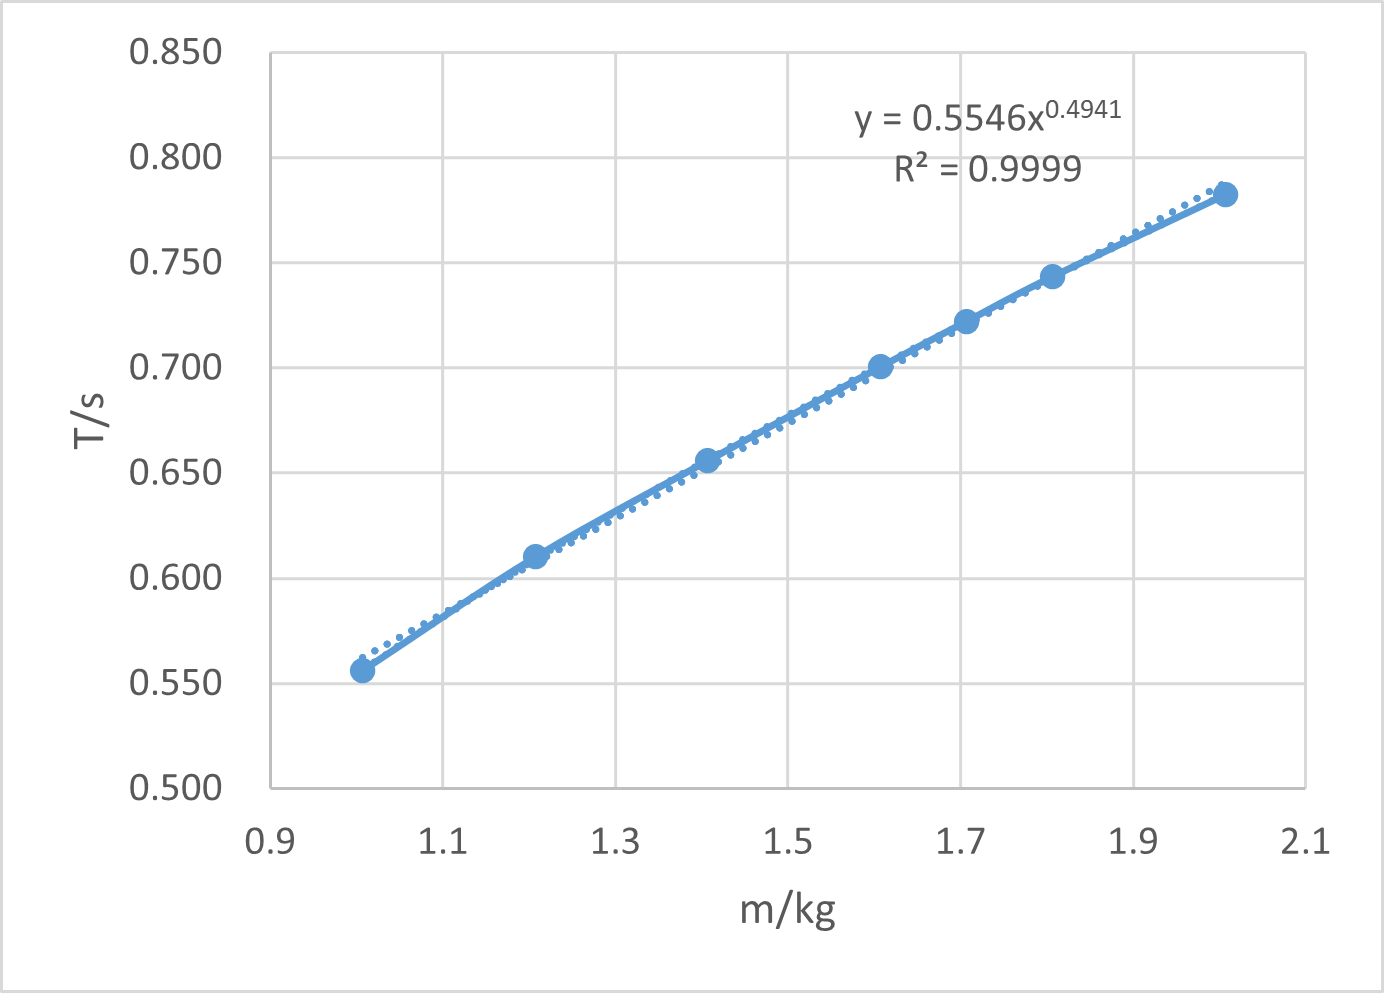
\includegraphics[width=.5\linewidth]{./fig/实验1指数.png}
	\caption{指数拟合 $T(m)$}\label{fig:实验1指数}
\end{figure}
使用 Excel 指数拟合结果 $y = 0.5546^{0.4941},R² = 0.9999$

为了进一步得到弹簧的弹性系数,对$F$与$x$的关系进行线性拟合,得到下表图

\begin{figure}[H]
	\centering
	\begin{minipage}{0.45\textwidth}
		\begin{table}[H]
			\centering
			\caption{弹簧伸长和受力关系}
			  \begin{tabular}{rrr}
			  \toprule
			  质量$M$(kg) &  距离$x$(m)& 力$F$(N)  \\
			  \midrule
			  1.0   & 0.446  & 9.8  \\
			  1.1   & 0.442  & 10.8  \\
			  1.2   & 0.430  & 11.8  \\
			  1.4   & 0.414  & 13.7  \\
			  1.6   & 0.400  & 15.7  \\
			  1.8   & 0.383  & 17.6  \\
			  2.0   & 0.367  & 19.6  \\
			  \bottomrule
			  \end{tabular}%
			\label{tab:实验一2计算k}%
		  \end{table}%
	\end{minipage}
	\begin{minipage}{0.45\textwidth}
		\centering
		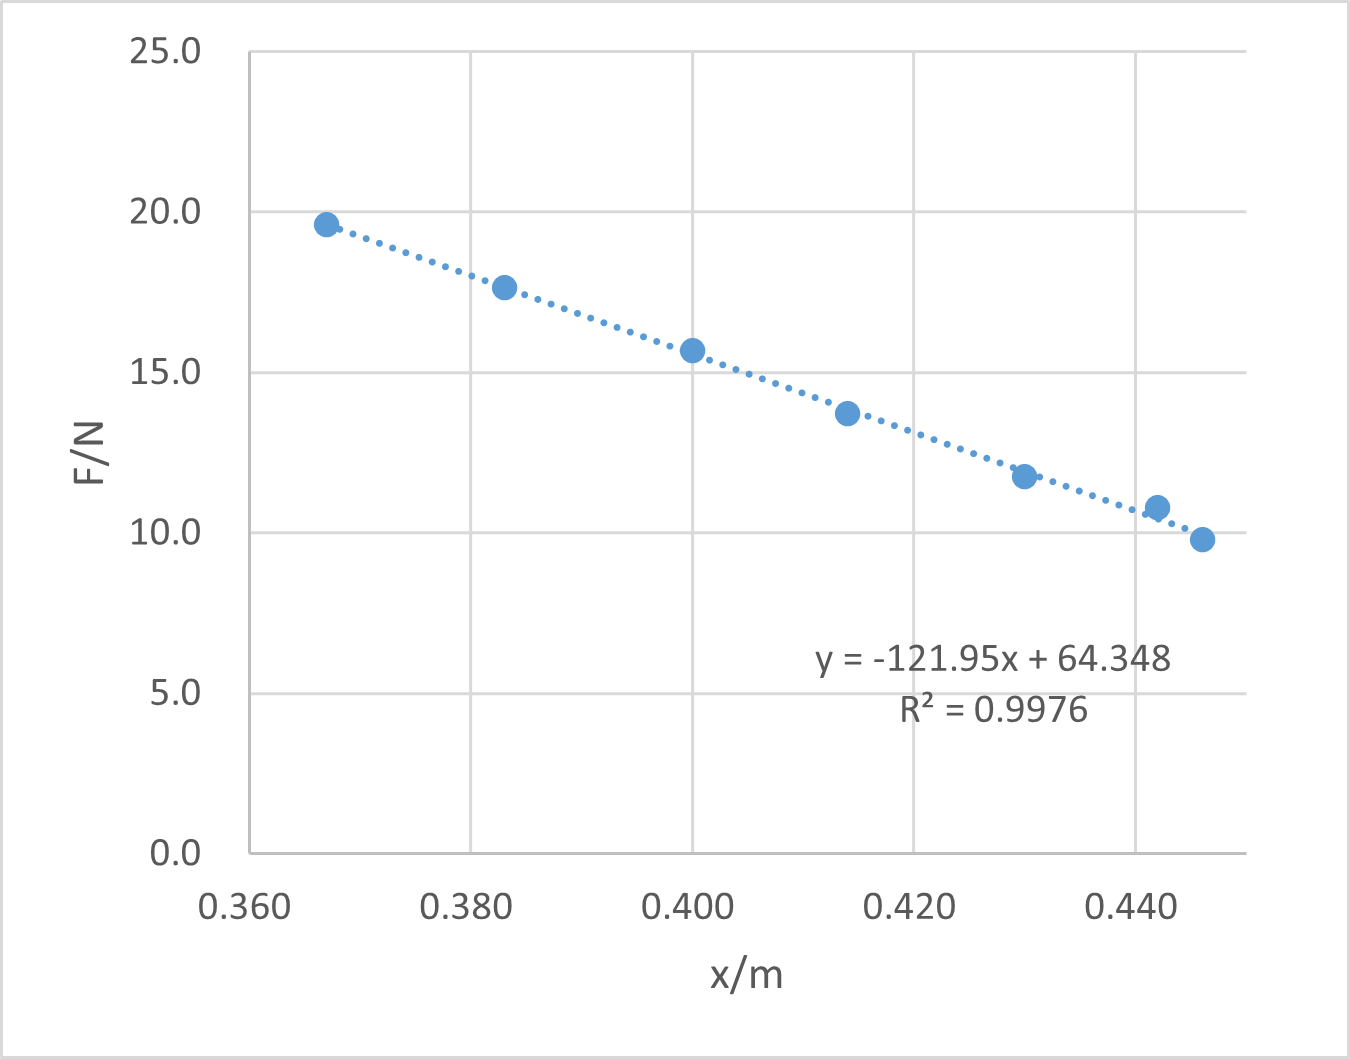
\includegraphics[width=\linewidth]{./fig/实验1直线.png}
	% 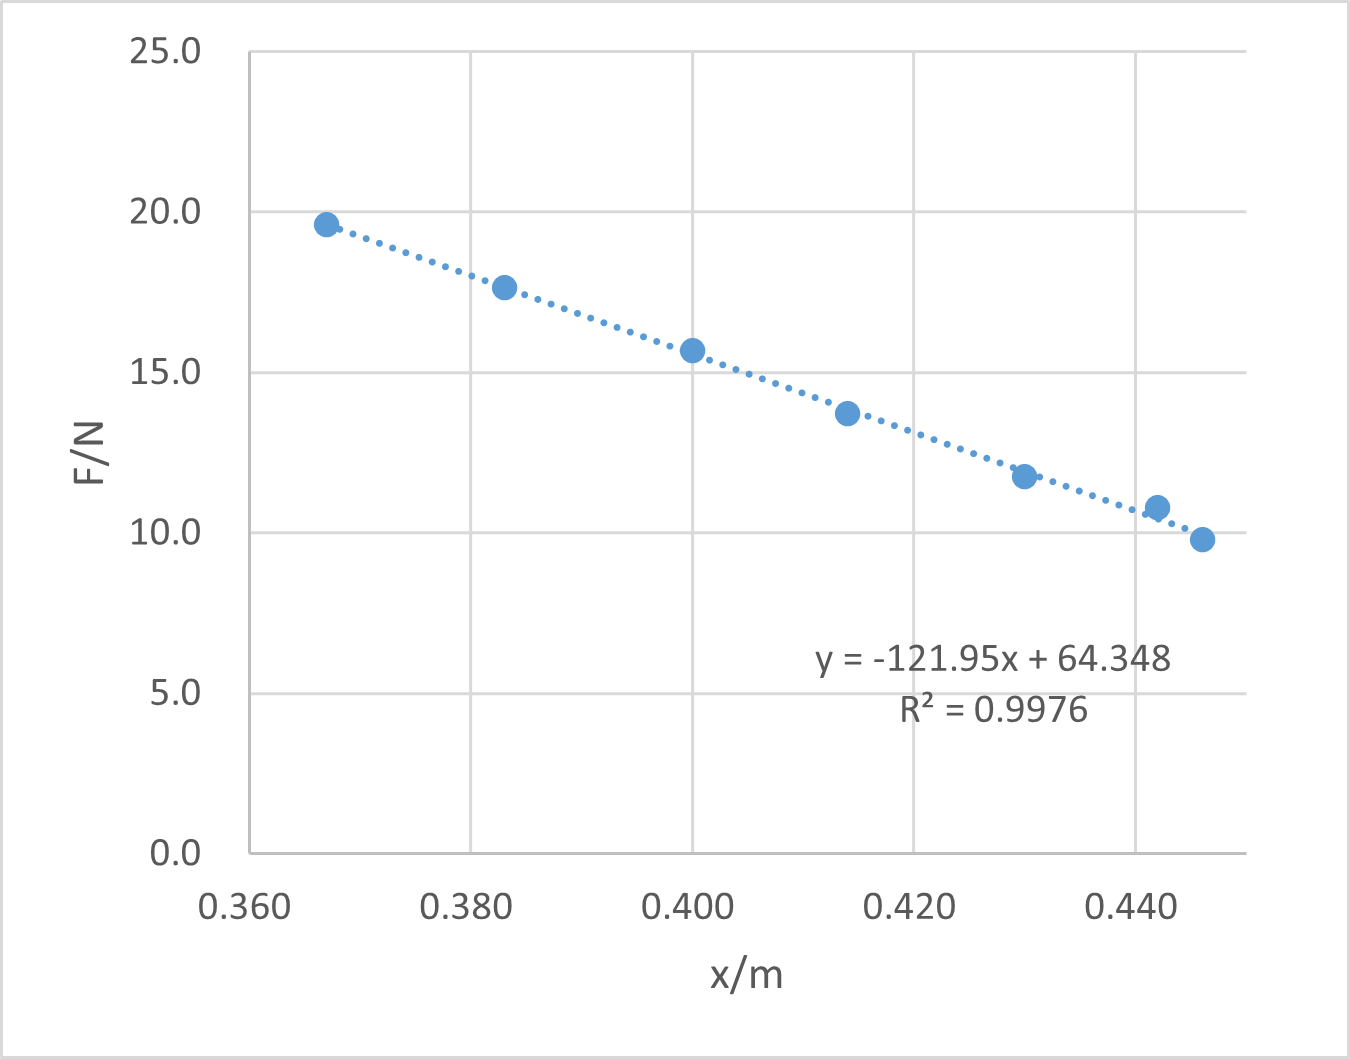
\includegraphics[]{./fig/实验1直线.png}
		\caption{弹簧弹力与位移关系}\label{fig:实验1直线}
	\end{minipage}
\end{figure}
使用 Excel 直线拟合结果 $y = -121.95x + 64.348,R² = 0.9976$,弹性系数为 $k=121.95$N/m

\subsection{控制$m$确定$T(k)$}
测量多个弹簧的弹性系数$k$,并选取一个质量$m$,对不同的弹簧使用Capstone 软件记录时间$t$对力$F$的图像,并使用正弦曲线拟合,记录拟合的频率$\omega$。
\paragraph{弹簧弹性系数$k$}
同上进行多次测量,得到数据下表:
\begin{table}[H]
	\centering
	\begin{subtable}{0.4\textwidth}
	\centering
		\begin{tabular}{rrrr}
			\toprule
			$M$(kg) & $m$(g) & $F$(N) & $x$(m) \\
			\midrule
			1.000  & 20.3990  & 9.866637 & 0.455  \\
			1.500  & 20.3990  & 14.76664 & 0.428  \\
			1.700  & 20.3990  & 16.72664 & 0.416  \\
			1.900  & 20.3990  & 18.68664 & 0.404  \\
			2.000  & 20.3990  & 19.66664 & 0.398  \\
			\bottomrule
		\end{tabular}
		\caption{甲}
	\end{subtable}
	\begin{subtable}[b]{0.4\textwidth}
		\centering
		\begin{tabular}{rrrr}
			\toprule
			$M$(kg) & $m$(g) & $F$(N) & $x$(m) \\
			\midrule
			0.500  & 7.5758  & 4.924748 & 0.420  \\
			0.700  & 7.5758  & 6.884748 & 0.385  \\
			0.900  & 7.5758  & 8.844748 & 0.344  \\
			1.000  & 7.5758  & 9.824748 & 0.330  \\
			1.200  & 7.5758  & 11.78475 & 0.286  \\
			1.400  & 7.5758  & 13.74475 & 0.252  \\
			1.500  & 7.5758  & 14.72475 & 0.231  \\
			\bottomrule
		\end{tabular}
		\caption{乙}
	\end{subtable}
	\begin{subtable}[b]{0.4\textwidth}
		\centering
		\begin{tabular}{rrrr}
			\toprule
			$M$(kg) & $m$(g) & $F$(N) & $x$(m) \\
			\midrule
			0.500  & 8.2180  & 4.926845 & 0.478  \\
			0.700  & 8.2180  & 6.886845 & 0.462  \\
			0.900  & 8.2180  & 8.846845 & 0.446  \\
			1.000  & 8.2180  & 9.826845 & 0.436  \\
			1.200  & 8.2180  & 11.78685 & 0.416  \\
			1.400  & 8.2180  & 13.74685 & 0.399  \\
			1.500  & 8.2180  & 14.72685 & 0.384  \\
			\bottomrule
		\end{tabular}
		\caption{丙}
	\end{subtable}
	\begin{subtable}{0.4\textwidth}
		\centering
		\begin{tabular}{rrrr}
			\toprule
			$M$(kg) & $m$(g) & $F$(N) & $x$(m) \\
			\midrule
			0.500  & 10.8193  & 4.935343 & 0.445  \\
			0.700  & 10.8193  & 6.895343 & 0.418  \\
			0.900  & 10.8193  & 8.855343 & 0.389  \\
			1.000  & 10.8193  & 9.835343 & 0.380  \\
			1.200  & 10.8193  & 11.79534 & 0.352  \\
			1.400  & 10.8193  & 13.75534 & 0.324  \\
			1.500  & 10.8193  & 14.73534 & 0.304  \\
			\bottomrule
		\end{tabular}
		\caption{丁}
	\end{subtable}
	\caption{测量弹簧弹性系数数据}
\end{table}

画图拟合:
\begin{figure}[H]
	\centering
	\begin{subfigure}{0.45\textwidth}
		\centering
		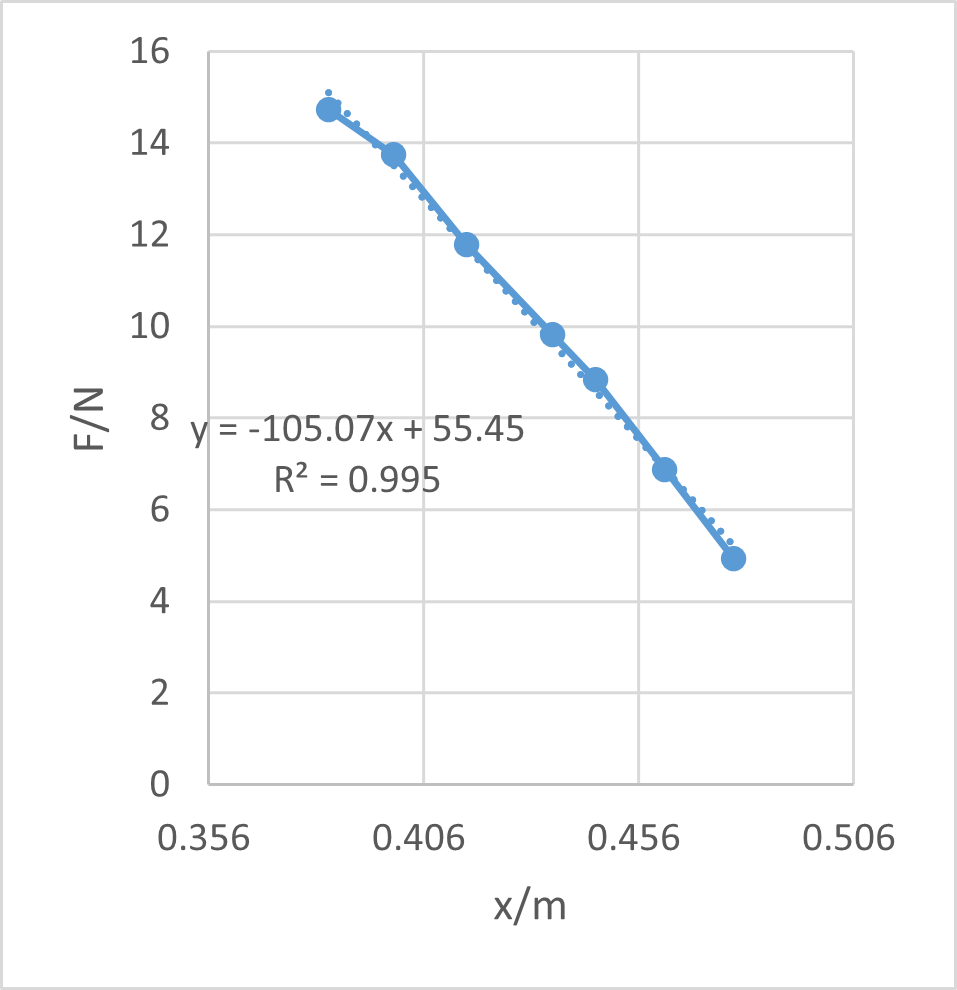
\includegraphics[width=\textwidth]{./fig/k105.png}
		\caption{甲}
	\end{subfigure}
	\begin{subfigure}{0.45\textwidth}
		\centering
		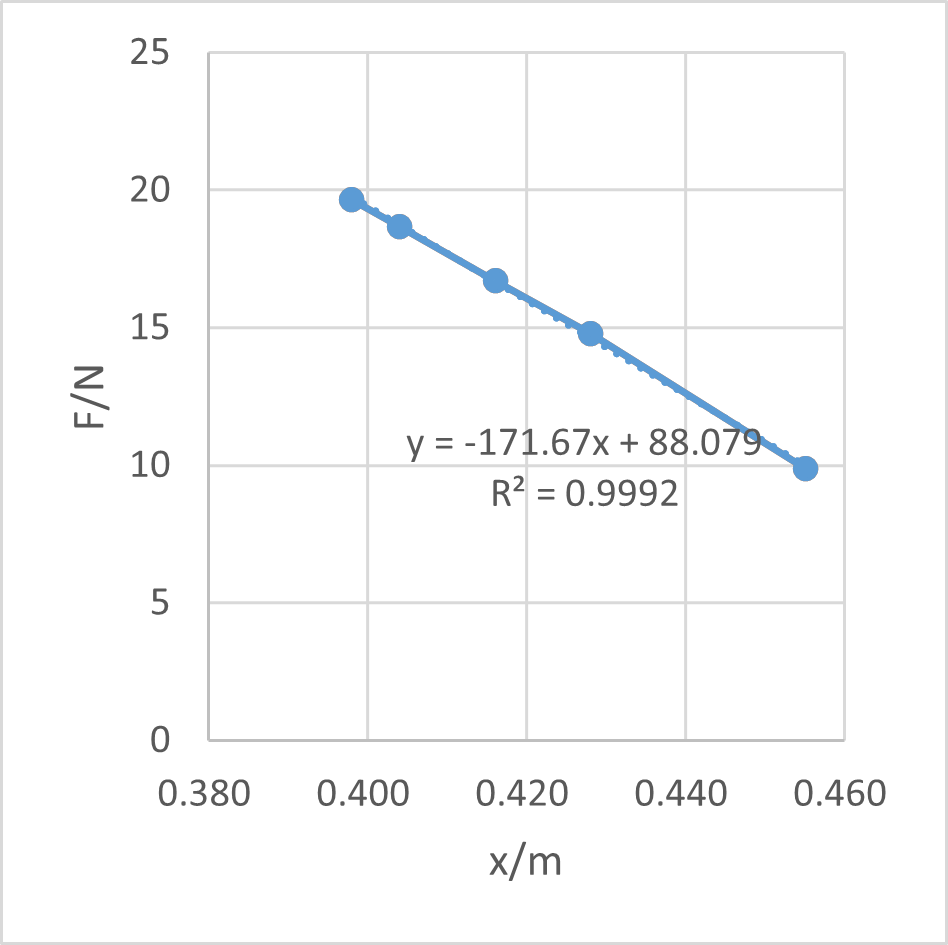
\includegraphics[width=\textwidth]{./fig/k171.png}
		\caption{乙}
	\end{subfigure}
	\begin{subfigure}{0.45\textwidth}
		\centering
		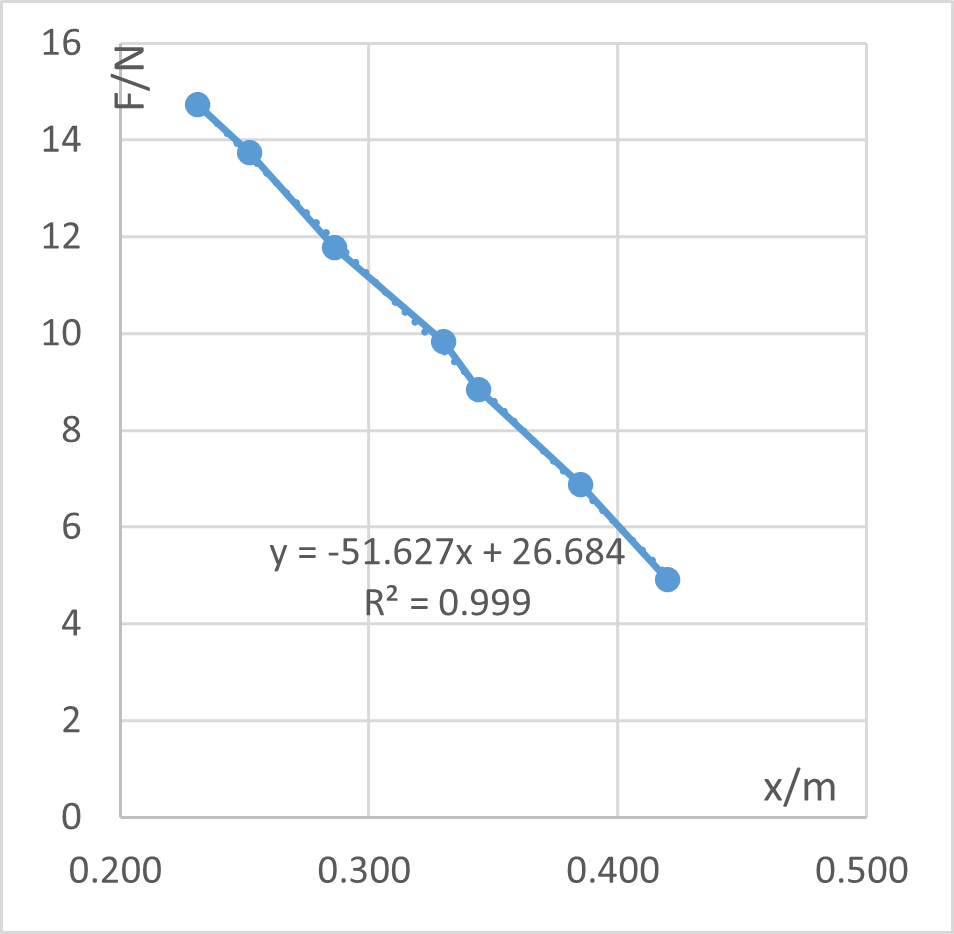
\includegraphics[width=\textwidth]{./fig/k51.png}
		\caption{丙}
	\end{subfigure}
	\begin{subfigure}{0.45\textwidth}
		\centering
		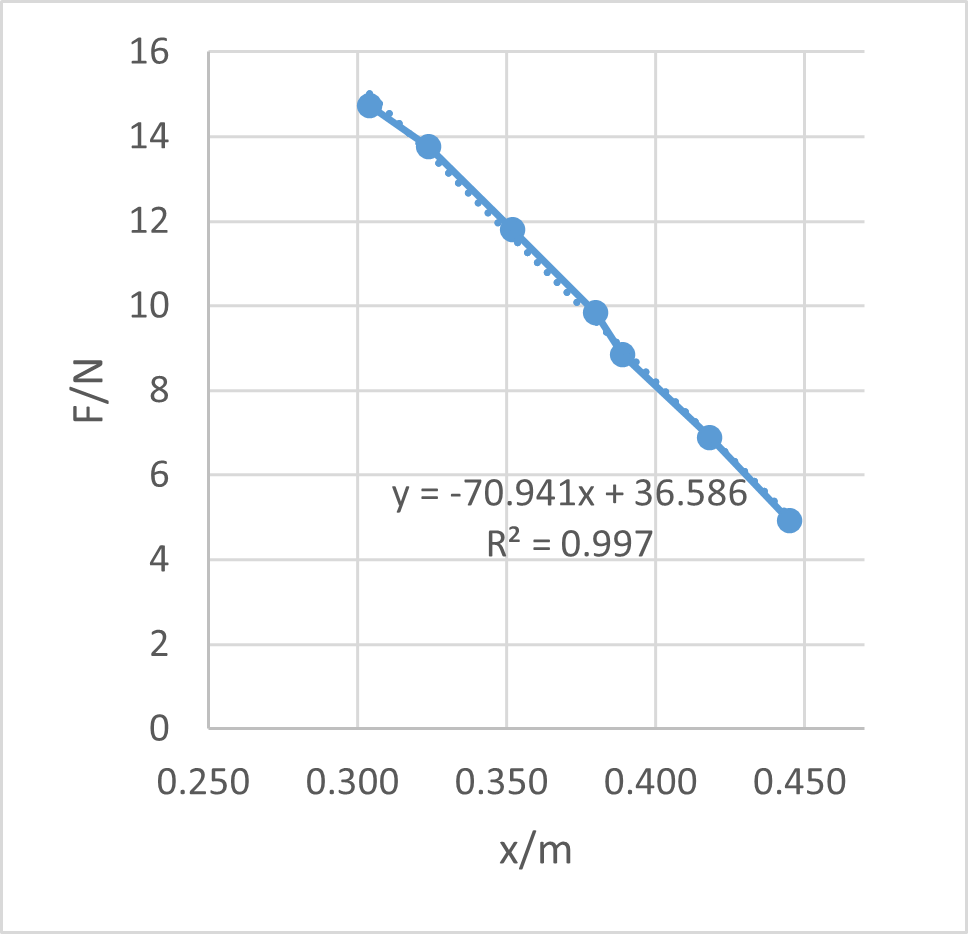
\includegraphics[width=\textwidth]{./fig/k70.png}
		\caption{丁}
	\end{subfigure}
	\caption{拟合结果}
	\label{fig:弹性系数}
\end{figure}
\paragraph{振动的周期}  
分别将五个弹簧挂上0.5kg砝码,轻轻拉动,计算震荡周期,得下表:
\begin{table}[H]
	\centering
	\caption{控制 m 记录 T 与 k 的关系}
	  \begin{tabular}{rrrr}
		\toprule
		角频率 $\omega$(rad/s) & 周期 $T$(s) & 弹性系数$k$(N/m) & 质量$M$(kg) \\
		\midrule
	  18.6  & 0.3378  & 171.67 & 0.5 \\
	  10.5  & 0.5984  & 51.537 & 0.5 \\
	  15.5  & 0.4054  & 105.07 & 0.5 \\
	  11.8  & 0.5325  & 70.941 & 0.5 \\
	  \bottomrule
	  \end{tabular}
	\label{tab:allk}
\end{table}
  
做出拟合结果
\begin{figure}[H]
	\centering
	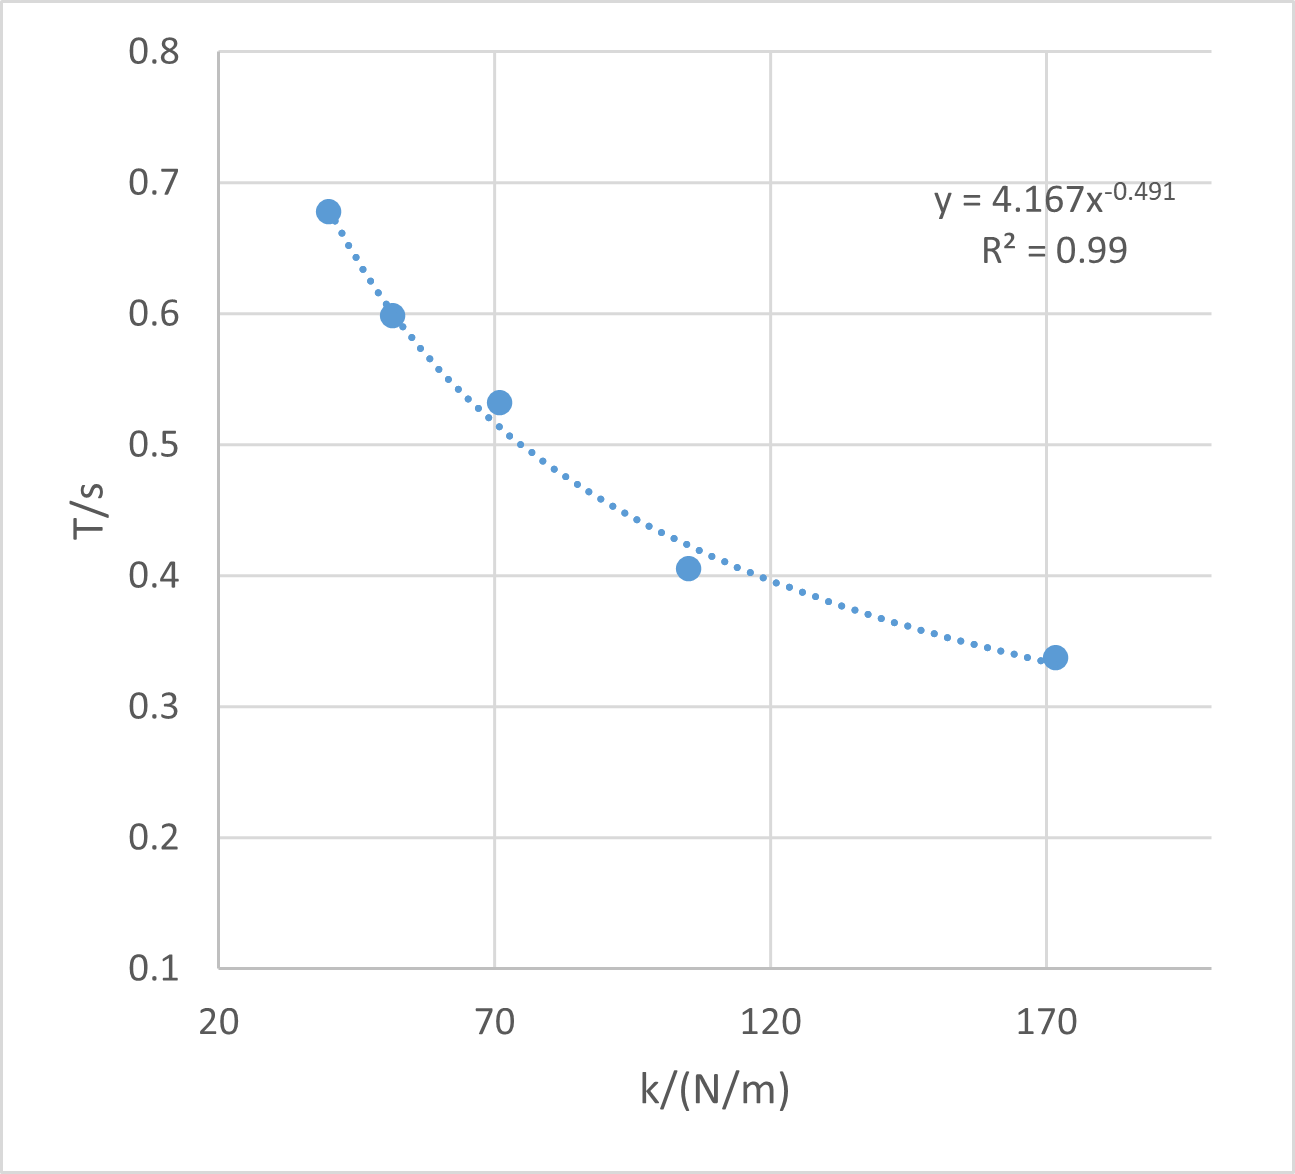
\includegraphics{./fig/实验2拟合.png}
	\caption{指数拟合 T(k)}
	\label{fig:}
\end{figure}

拟合曲线为 $y = 4.167 x^{-0.491},R² = 0.99$,幂次为$-0.491$

可能是由于硬度最大的弹簧未拉开,硬度最小的弹簧拉太长,均离开线性区导致。之后考虑是弹性系数测量不够精准导致。

\subsection{量纲分析}
按照原理中指出一般方法:
\begin{enumerate}
	\item 相关变量:周期$T$、质量$m$、劲度系数$k$。
	\item 构造关系式$T=f(m,k)$。
	\item 寻找无量纲组合:利用量纲分析,我们可以推导出,要使$T$、$m$、和$k$的关系式的量纲一致,可能的组合是$\sqrt{m/k}$,因为其量纲是$\sqrt{[M]/([M/T^2])}=[T]$。
\end{enumerate}

因此,我们可以推测$T=C\sqrt{m/k}$,其中$C$由解力学方程为$2\pi$。

\subsection{求解T(m,k)解析式}

两个实验分别得到
\begin{align*}
	T & = 0.5546m^{0.4941}\\
	T & = 4.167 k^{-0.491}
\end{align*}
约去控制变量时未改变的$m$/$k$值,可计算常数$C$。

代入 $m=0.5\text{kg},k=-121.95\text{N/m}$对于$T(m,k)$:
\begin{align}
	C_m &= \frac{0.5546}{121^{-0.491}}=5.93\\
	C_k &= \frac{4.167}{0.5^{0.4941}}=5.86
\end{align}

则可得$C$的测量值为
\begin{equation}
	C= \frac{C_m+C_k}{2}=\frac{5.93+5.86}{2}=5.90
\end{equation}

则最终所得$T(m,k)$为

\begin{equation}
	T(m,k) = 5.90 \frac{m^{0.4941}}{k^{0.491}}
	\label{eq:tmk}
\end{equation}

\subsection{误差分析}
\subsubsection{相对误差}
实验计算出的误差与理论公式$T=2\pi \sqrt{\frac{m}{k}}$略有偏差,计算相对误差得
\begin{align}
	E_C & = \frac{\left|5.90-2\pi\right|}{2\pi} \times 100\% = 6.1\%                \\
	E_m & = \frac{\left|0.4941-0.5\right|}{0.5} \times 100\% = 1.18\%   \\
	E_k & = \frac{\left|-0.491+0.5\right|}{-0.5} \times 100\% = 1.8\%
\end{align}

\subsubsection{误差来源}
\paragraph{偶然误差}
\begin{itemize}
	\item 长度测量误差测量弹簧伸长量时,可能因硬纸片的位置倾斜引起测量误差。
	\item 弹簧晃动,不只垂直晃动,在水平方向上发生位移,导致测量的周期不准确。
\end{itemize}

\paragraph{系统误差}
\begin{itemize}
	\item 弹簧的弹性限度,弹簧超出其弹性限度后,行为可能不再符合胡克定律,超出线性区,伸长量与弹力不成线性关系。
	\item 摩擦和阻力,空气阻力和支架上的摩擦可能影响振动周期。
	\item 弹簧非均匀振动,不同部分的振动存在差异。
	\item 弹簧非理想性,弹簧在多次使用后微微变形,弹性变化。
\end{itemize}

\subsubsection{减小误差方法}
为了减少误差,实验过程中可以采取以下措施:
\begin{itemize}
	\item 测量多个周期的平均值,确保拟合不变。
	\item 弹簧的伸长量测量时减少测量误差。
	\item 多次测量弹簧弹性系数。
	\item 控制弹簧不超过其弹性限度。
	\item 保持支架稳固不要水平晃动。
\end{itemize}

% \longLine
\section{实验结果陈述与总结}
\subsection{结果陈述}

根据实验数据与拟合曲线,得到:周期 \(T\) 与质量 \(m\) 的关系符合 \(T = C_1 \cdot \sqrt{m}\),实验拟合指数0.4941;与弹性系数 \(k\) 的关系满足 \(T = C_2 \cdot \frac{1}{\sqrt{k}}\),实验拟合指数 0.491。
实验数据与量纲分析理论预测一致,指数误差为$E_m=1.18\%,E_k=1.8\%$,综合理论结果为 $T=2\pi\sqrt{\frac{m}{k}}\sim 2\pi\frac{m^{0.4941}}{k^{0.491}}$

\subsection{实验总结}

通过这个实验,学到了运用控制变量法,量纲分析法来研究物理现象,验证了周期与质量平方根和劲度系数平方根的关系。加深对简谐振动的理解,再次熟悉在收集数据和分析图表技能。通过这样一个实验,我学习到了如何对物理现象进行研究,发掘它的规律的方法,有了很大提高。同时看到其它同学完美的$R^2=0.9999$和更好地拟合出平方根结果,知道自己还需要精益求精。

\endBox
\end{document}
